%%%%%%%%%%%%%%%%%%%%%%%%%%%%
% CHAPTER 7 - DISCUSSION of THEORY: CROSS-TOOL
%%%%%%%%%%%%%%%%%%%%%%%%%%%%
%%%%%%%%%%%%%%%%%%%%%%%%%%%%%%%%%%%%%%%%%%%%%%%%%%%%%%%%%%%%%%%%%%%%%%%%%%%%%%%%%%%%%%%%%%
% Richard Boardman PhD Thesis: Improving Tool Support for Personal Information Management
%%%%%%%%%%%%%%%%%%%%%%%%%%%%%%%%%%%%%%%%%%%%%%%%%%%%%%%%%%%%%%%%%%%%%%%%%%%%%%%%%%%%%%%%%%
% Towards a more realistic/alternative cross-tool model of today's workspace and user's PIM activity to understand/discuss -- parallel management of multiple PIM systems.  A new way of seeing problem/ a new perspective. Raises both opportunities and challenges. 

%%%%%%%%%%%%%%%%%%%%%%%%%%%
\subsection{PIM as a Cross-tool Activity}
\label{discussion:cross-tool}
%%%%%%%%%%%%%%%%%%%%%%%%%%%
%%%%%%%%%%%%%%
% CROSS-TOOL
%%%%%%%%%%%%%%
%\textbf{Definition of workspace. Starting analytical scope.}
%		\item Space as environment
%		\item Physical and digital
%		\item Relate to Kirsh's work context
%		\item Location for production and supporting activities
%%%%%%%%%%%%%%%%%%%%%%%%%%%%%%%%%%%%%%%%%%%%%%%%%%%%%%%%%%%%%%%%%%%%%%%%%%%%%%%
%		\item Abstract PIM system. DIAGRAM (as in Kaptelinin)
%		\item Here the computer as a PIM system cf. specific tools as PIM systems
%%%%%%%%%%%%%%%%%%%%%%%%%%%%%%%%%%%%%%%%%%%%%%%%%%%%%%%%%%%%%%%%%%%%%%%%%%%%%%%
% Workspace as a cross-tool artifact to support cross-tool PIM activity (THINK: how would Carroll talk about it all?). Feature as an artifact? (REF: Raskin) From PIM-tool as habitat to workspace as habitat
% HOW TO FRAME AS INITIAL FOCUS?
% -- since tools are inter-related
% Evidence: problems, activities are cross-tool (from chapter 4)
%%%%%%%%%%%%%%%%%%%%%%%%%%%%%%%%%%%%%%%%%%%%%%%%%%%%%%%%%%%%%%%%%%%%%%%%%%%%%%%
% Firstly, evidence from earlier chapters is presented to support this view.  Then, Barreau's model of PIM~\citep{barreau:95} is extended to encompass the cross-tool nature of PIM.  This model is contrasted with related theoretical views. Building on the model presented in \textbf{Section~\ref{discussion:cross-tool:activity-model}}, a model of PIM strategies is proposed to reflect the empirical findings reported in \textbf{Chapters~\ref{chapter:exploratory_study}} and \textbf{\ref{chapter:main-study}}.  Finally, implications for design and methodology are discussed. Two analytical perspectives are discussed, the computer workspace as (1) a single PIM artefact, and (2) a set of parallel PIM artefacts.  

%%%%%%%%%%%%%
% OVERVIEW
%%%%%%%%%%%%%
% This section discusses PIM from the first of three theoretical perspectives: that of PIM as a \textit{cross-tool} activity (one that involves multiple tools).

%%%%%%%%%%%%%%%%
% EVIDENCE
%%%%%%%%%%%%%%%%
%%%%%%%%%%%%%%%%%%%%%%%%%%%%%%%%%%%%%%%%%%%%%%
%\subsection{Evidence for cross-tool view}
%\label{discussion:cross-tool:evidence}
%%%%%%%%%%%%%%%%%%%%%%%%%%%%%%%%%%%%%%%%%%%%%%
% FOUNDATION: cross-tool data, evidence of PIM CT problems etc.
% Highlight findings from Literature Review and exploratory study that motivate/justify this approach.
% Information Management and Task Management are distributed. DIAGRAM.
Today's computing environments allow users to manage information in a variety of PIM-tools.  However, as noted in \textbf{Chapter~\ref{chapter:review}}, most previous PIM studies have focused on specific tools such as files or email.  In contrast, this research employed a deliberately cross-tool approach to investigate ways of improving integration between PIM-tools.  A focus was taken on three PIM-tools: files, email and bookmarks.  Almost all of the study participants from \textbf{Chapters~\ref{chapter:exploratory_study}} and \textbf{\ref{chapter:main-study}} actively managed all three PIM-tools.  The observations of \textit{folder overlap} indicate the information relating to a particular activity was fragmented across PIM-tools.  In other words. multiple PIM-tools were involved in certain user activities.  Also, the management of information in a particular technological format (e.g. files), was \textit{compartmentalized} across different PIM-tools.

These observations lead the author to conceptualize PIM as a \textit{cross-tool} activity, one that is distributed across multiple tools.  Previous tool-specific research in the context of email, has considered how the collection of messages acts as a \textit{``habitat''} for user activities~\citep{Ducheneaut:01}.  In contrast, this section considers PIM from a cross-tool perspective, whereby email is one component of the wider habitat of the user's personal information environment. %a user's cross-tool activity space. 

% A key driver behind this thesis work was to investigate PIM from a crss-tool perspective, and in particular to investigate the potential to improve integration between PIM-tools.  The research focused on three commonly-employed PIM-tools: files, email and bookmarks.
% The observation of folder overlap in \textbf{Section~\ref{exp-study:Results-folder-overlap}} indicate that multiple PIM-tools are utilised in specific user activities and roles.  
% Therefore, the view is taken that PIM is 
% \textbf{Chapter~\ref{chapter:exploratory_study}} reports a cross-tool study. \textbf{Chapter~\ref{chapter:design}} outlines the design of WorkspaceMirror (WM), a mechanism to integrate how information is organized in three PIM-tools.  \textbf{Chapter~\ref{chapter:main-study}} reports a second cross-tool study centred on the evaluation of the WM prototype. % REFER TO OTHER RELATED WORK/FINDINGS.
%%%%%%%%%%%%%%%%%%%%%%%%%%%%%%
% \subsubsection{Related work}
% \label{discussion:cross-tool:related-theory}
%%%%%%%%%%%%%%%%%%%%%%%%%%%%%%
% Evidence from studies of cross-tool'ness, problems etc. (Blandford and Green (harmonious co-mingling), Bellotti)
% Based on findings from literature review and my own data/experience.  Theoretical motivation, similar stances:
Various strands of related research come together in supporting this perspective.
%%%%%%%%%%%
% KIRSH
%%%%%%%%%%%
% Distributed Cognition (space/people, time, internal/external). Kirsh's view of work context ~\cite{dk:00}. Computer as an activity space containing resources and constraints
In terms of theory, the view draws on the conceptualization of a computer as an \textit{activity space}, populated by the tools and resources that facilitate action, and the constraints that limit it~\citep{dk:01}. From this theoretical perspective, activities such as PIM, are not confined to specific tools, but are distributed across a range of tools throughout digital activity space.
%%%%%%%%%%%%%%%%%%%%%%%%
% BLANDFORD AND GREEN
%%%%%%%%%%%%%%%%%%%%%%%%
Recent empirical work has also highlighted how the management of certain types of information is fragmented across multiple PIM-tools, e.g. to-dos and appointments~\citep{bg:01,Bellotti:00}, bookmarks~\citep{kftf:01}, and contacts~\citep{Whittaker-contacts:02}.  % \citet{bg:01} offer the term \textit{ensemble} to describe the set of tools that task and time management are distributed across.


%%%%%%%%
% BELLOTTI ET AL.
%%%%%%%%
% In order to provide effective support for such cross-tool activities, integration between tools is crucial. However there is evidence that this issue is not being given enough attention by designers. Bellotti and Smith (2000) note the compartmentalization of PIM activities due to poor integration between tools. For example, document collections are often divided between those stored in the file system and those stored as email attachments.
%%%%%%%%%%%%%%%%%%%%%%%%%%%%%%%%%%%%%%%%%%%%%%%%%%%%%%%%
% USE ME:In terms of the theoretical framework offered by Kirsh, compartmentalization may be considered as one set of constraints imposed on a user's activity space by poorly designed tools.
%%%%%%%%%%%%%%%%%%%%%%%%%%%%%%%%%%%%%%%%%%%%%%%%%%%%%%%%
%%%%%%%%
% DIX
%%%%%%%%
%\textit{Dix ~\cite{dix:98} (but focus on coordinating)}
%%%%%%%%%%%%%%%%%%%%%%%%%%%%%%%%%%%%%%%%%%%%%%%%%%%%%%%%
%%%%%%%%%%%%%%%%%
% KAPTELININ
%%%%%%%%%%%%%%%%%
%\textit{Kaptelinin~\citep{Kaptelinin:96,Kaptelinin:03} -- model of PIM activity}
%%%%%%%%%%%%%%%%%%%%%%%%%%%%%%%%%%%%%%%%%%%%%%%%%%%%%%%%
%%%%%%%%%%%%
% Raskin
%%%%%%%%%%%%
%\textit{Relate to Raskin. Content as content with standard operations.}
%\textit{Here, it is argued that PIM support is a cross-tool feature set.  Unified amalgam of all PIM functionality.}
%%%%%%%%%%%%%%%%%%%%%%%%%%%%%%%%%%%%%%%%%%%%%%%%%%%%%%%%
%%%%%%%%%%%%%%%%%%%%%%%%%%%%%%%%%%%%%%%%%%
% What are limitations of this theory?
% i.e. why am I even trying to do this?
%%%%%%%%%%%%%%%%%%%%%%%%%%%%%%%%%%%%%%%%%%
%\textit{What is wrong with existing models/are there any?}
%%%%%%%%%%%%%%%%%%%%%%%%%%%%%%%%%%%%%%%%%%%%%%%%%%%%%%%%

%%%%%%%%%%%%%%%%%%%%%%%%%%%%%%%%%%%%%%%%%%%%%%%%%%%%%%%%%%%%%%%%%%%%%
\subsubsection{Extending the Conceptual Framework from Chapter 2}
%%%%%%%%%%%%%%%%%%%%%%%%%%%%%%%%%%%%%%%%%%%%%%%%%%%%%%%%%%%%%%%%%%%%%

%%%%%%%%%%%%%%%%%%%%%%
% BUILD ON BARREAU
%%%%%%%%%%%%%%%%%%%%%%
% However here it is argued that such an abstract view does not accurately reflect the nature of the PIM carried out by today's users.
% Now want to shift boundaries based on a new analytical perspective.  Idea of a model which tool designers can refer to. Or better as just simple recommendations?
% The workspace as a PIM-tool.  PIM as a cross-tool activity. 
% Here we go -- a Cross-Tool Analytical Proto-Model of Cross-tool PIM}:
% Cue cross-tool model of workspace (REF: a la Victor's model) 
% Barreau's framework~\citep{barreau:95} is extended to reflect the workspace as a high-level PIM system, containing lower-level PIM systems within distinct tools.  
% \textbf{Chapter~\ref{chapter:bg}} provided a brief introduction to Barreau's model of PIM, consisting of four sub-activities: acquisition, organization, maintenance and retrieval.
\textbf{Chapter~\ref{chapter:bg}} presented a conceptual framework of four PIM sub-activities: acquisition, organization, maintenance and retrieval. This was based on ~\citet{barreau:95} who models the computer as a \textit{single PIM system}.  % However, as discussed above, today's computers offer the facility to manage multiple collections of information, based on distinct technological formats, within different PIM-tools.
Here it is argued that another more accurate conceptualization of a personal computer is as a \textit{set of distinct PIM-systems}\footnote{Barreau's abstraction of the computer as a single PIM system may be due to the fact that her work was focused on the file system, and furthermore was carried out in 1995.  Other PIM-tools, such as email and web browsers were not as common then as now. Indeed, Barreau notes that only two of her eight participants managed email.}.
%%%%%%%%%%%%%%%
% NEW MODEL
%%%%%%%%%%%%%%%
\textbf{Figure~\ref{fig:discussion:PIM-cross-tool-model}} illustrates the extension of Barreau's framework to reflect this view.  PIM can therefore be viewed from two perspectives as follows:
%The primary reason for the limitations of Barreau's model is that her study focused on one tool: the file system.  The author acknowledges that this is an understandable limitation, since in 1995, .  % Indeed in 1995, when her study was reported, few participants employed email, and web browsers were not common.  Barreau conceptualized the computer as a single abstract PIM system, whereas from our data it is clear that current PIM-tools constitute a set of parallel yet inter-related systems. We also seek to modify the framework to capture the influence of production tasks in determining PIM needs.

\begin{enumerate}

%%%%%%%%%%%%%%%%%%%%%%%
% UNIQUE SUB-SYSTEMS
%%%%%%%%%%%%%%%%%%%%%%%
%Each tool allows the user to manage a specific type of information, in other words they amount to a specific PIM-system.  
% Why do we need to consider different aspects of each PIM sub-system?
% PIM has unique qualities in some tools.  In other words, PIM as an abstract activity that is instantiated in multiple PIM tools, possibly in slightly different ways. Some information in tools is self-contained. Other aspects overlap.
\item Firstly, from a \textit{tool-specific} perspective, each PIM-tool can be considered as a distinct PIM system which provides the functionality to acquire, organize, maintain and retrieve information based on a specific technological format. Although different PIM-tools share commonalities, they also have many unique aspects. \textbf{Chapter~\ref{chapter:exploratory_study}} surveyed how the nature of the PIM sub-activities varied across files, email and bookmarks. % could use example of acquisition here

%%%%%%%%%%%%%%%%%
% INTEGRATION and link to next section
%%%%%%%%%%%%%%%%%
Linking the independent ``PIM-subsystems'' are \textit{integration mechanisms}, such as email attachment functionality, and the WM prototype proposed in \textbf{Chapter~\ref{chapter:design}}.

%%%%%%%%%%%%%%%%%%%%%%%%%%%%%%%%%%%%%%%
% HL global system
% Set of sub-systems
% I.e. look beyond individual tools. 
%%%%%%%%%%%%%%%%%%%%%%%%%%%%%%%%%%%%%%%
% If to consider the computer as single PIM system, it must be recognised that it is made up of multiple PIM sub-systems. Different PIM-tools contribute together to high-level PIM support afforded by the workspace as a whole.  Treat as workspace-wide phenomena/workspace-level. Represents change from application-centric view
% Multiple PIM sub-systems that amount together to a computer-wide PIM-system.   
% Acquisition into ``global PIM system'' is net effect of all the parallel tool-specific acquisition.  Sources of PI: self-created, sent/pushed, actively seeking/foraged).
\item Secondly, from a \textit{cross-tool} perspective, the entire desktop computer can be considered as one federated PIM system composed of the set of tool-specific PIM sub-systems.  From a cross-tool perspective, the acquisition sub-activity is the sum of all the tool-specific acquisition processes, including email messages received from other people, and files and bookmarks created by the user.

\end{enumerate}  


% %%%%%%%%%%%%%%%%%%%%%%%%%%%%%
% FIGURE - Cross-tool ACTIVITY model of PIM
% %%%%%%%%%%%%%%%%%%%%%%%%%%%%%
%%%%%%%%%%%%%%%%%%%%%%%%%%%%%%
\begin{figure}[htbp]
	\begin{center}
		\leavevmode
		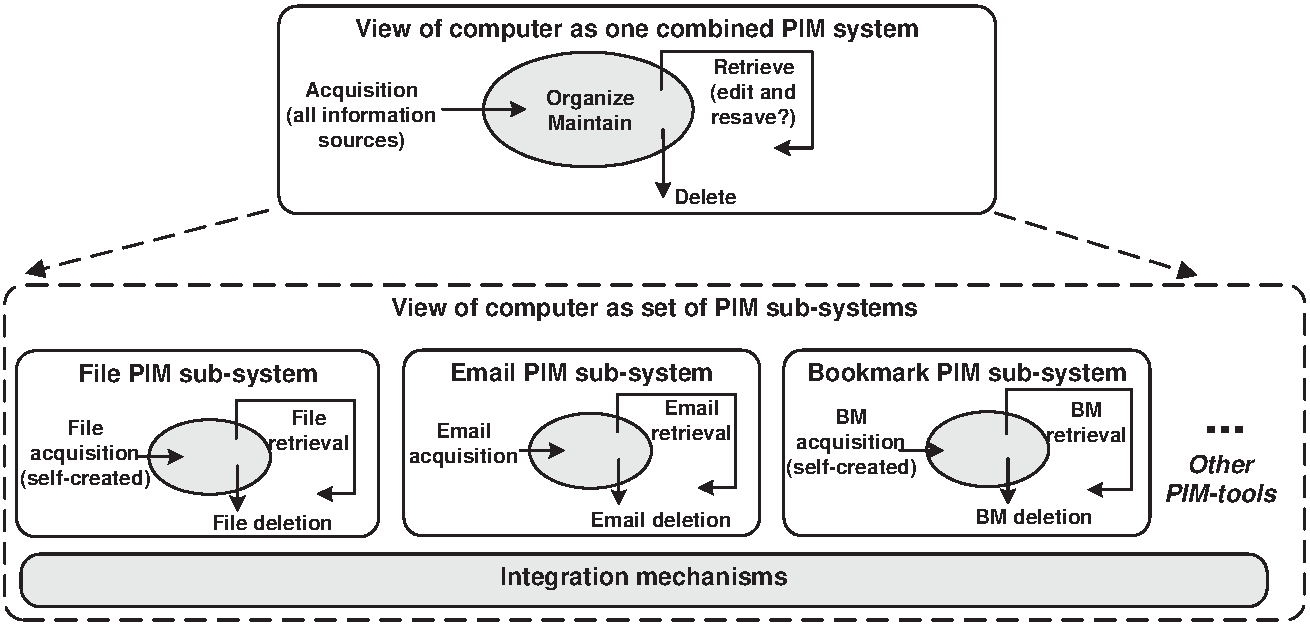
\includegraphics[width=\textwidth]{pictures/discussion/PIM-cross-tool-model.pdf}
		% fs-fm-comparison.pdf}
	\end{center}
	\caption{An extension of Barreau's PIM framework to reflect the cross-tool perspective}
	\label{fig:discussion:PIM-cross-tool-model}
\end{figure}



%%%%%%%%%%%%%%%%%%%%%%%
% TIP OF THE ICEBERG
%%%%%%%%%%%%%%%%%%%%%%%
% But also can consider far beyond the desktop
% Need to think beyond desktop as well - what about extended workspace?  
% There are many others, for example on the desktop, calendars, remote file stores and to-do-lists.  There are also other devices that should be considered, although outside the scope of this research programme.
% Note that the figure only includes three example PIM-tools, there are many more. One can also imagine a more extensive abstract view of the extended personal information environment.
\textbf{Figure~\ref{fig:discussion:PIM-cross-tool-model}} is limited to a focus on three PIM-tools: files, email and bookmarks.  However, these three are intended as indicative examples only.  Other PIM-tools could be included such as calendars and to-do lists.  Future extensions could also consider the extended personal information environment beyond the desktop -- shared drives, web-based information, as well as information stored on other devices and in the physical environment.  For now, the point to be taken by the reader is that PIM can be considered as a cross-tool activity.
% Also, many other tools have PIM facilities, even tools not really thought of as PIM tools.  


%%%%%%%%%%%%%%%%%%%%%%%%%%%%%
% LINK TO NEXT SECTIONS
%%%%%%%%%%%%%%%%%%%%%%%%%%%%%
% Before moving onto design implications,
The key benefit of the extended framework is that it allows the accommodation of cross-tool integration mechanisms.
\textbf{Section~\ref{discussion:supporting}} moves on to further develop the framework in \textbf{Figure~\ref{fig:discussion:PIM-cross-tool-model}} to encompass the relationship between PIM and the production tasks that it supports.

%%%%%%%%%%%%%%%%%%%%%
% FIN: CROSS-TOOL
%%%%%%%%%%%%%%%%%%%%%







